\clearpage
\newpage
\section{Additional Experiments on Run Time}
\label{app:runtime}

We include additional experiments comparing the run time of different clipping approaches.
Our goal is to further consolidate the claims that 1) adaptive per-layer clipping attains similar or better task performances under the same epoch budget for certain workflows, and that 2) this translates into compute time savings since per-layer clipping is faster than alternative clipping approaches per update (or almost equivalently per epoch).
All experiments here are performed on a machine with a single Titan RTX GPU with 24 GB of VRAM (different from the configuration in Figure~\ref{fig:throughput-comparison} which uses a single A6000 GPU).

The direct experiment we perform is to full fine-tune GPT-2 on E2E with three clipping approaches (adaptive per-layer, ghost, and flat clipping) under the same epoch constraint (which we fix to be 10 for all workflows).
Regarding hyperparameters for flat clipping, we adopt the set of values obtained from extensive tuning on this task used by~\cite{li2022large}.
We reuse the same set of hyperparameters values for ghost clipping, since the approach essentially results in the same gradient updates as flat clipping up to numerical precision (only computed in a different way).
Using these near optimal hyperparameters for flat and ghost clipping prevents our experiments from unfairly disfavouring the two approaches.
Figure~\ref{fig:gpt2runtime-overall-nll} shows that adaptive per-layer clipping consistently achieves lower test set negative log-likelihood than flat clipping and ghost clipping under any given wall time elapse.
While language generation metrics (e.g., BLEU and ROUGE-L) are generally noiser than the test set NLL, Figure~\ref{fig:gpt2runtime-overall-task-metric} shows that adaptive per-layer clipping generally yields better task metric numbers compared to flat clipping and ghost clipping under the same wall time.

Finally, we note the caveat that the precise run time advantage of adaptive per-layer clipping against flat clipping may vary across machines and GPU types.
In addition, the realized gains for actual training workflows might be smaller than that observed in our controlled experiments (e.g., Figure~\ref{fig:throughput-comparison}) due to compute time spent on auxiliary operations such as data loading and data preprocessing (e.g., pad sequences of different length to the same length). 
For instance, we repeat the controlled experiment in Figure~\ref{fig:throughput-comparison} but this time with a different GPU, and observe slightly different factors of speed gains. 
Overall, we generally see that adaptive per-layer clipping is above 1.4x the speed of flat clipping in our controlled experiments, and the realized gains is roughly as much for full fine-tuning on E2E with our implementation.

\begin{figure}[htb]
\begin{center}
\begin{minipage}[t]{0.5\linewidth}
\centering
{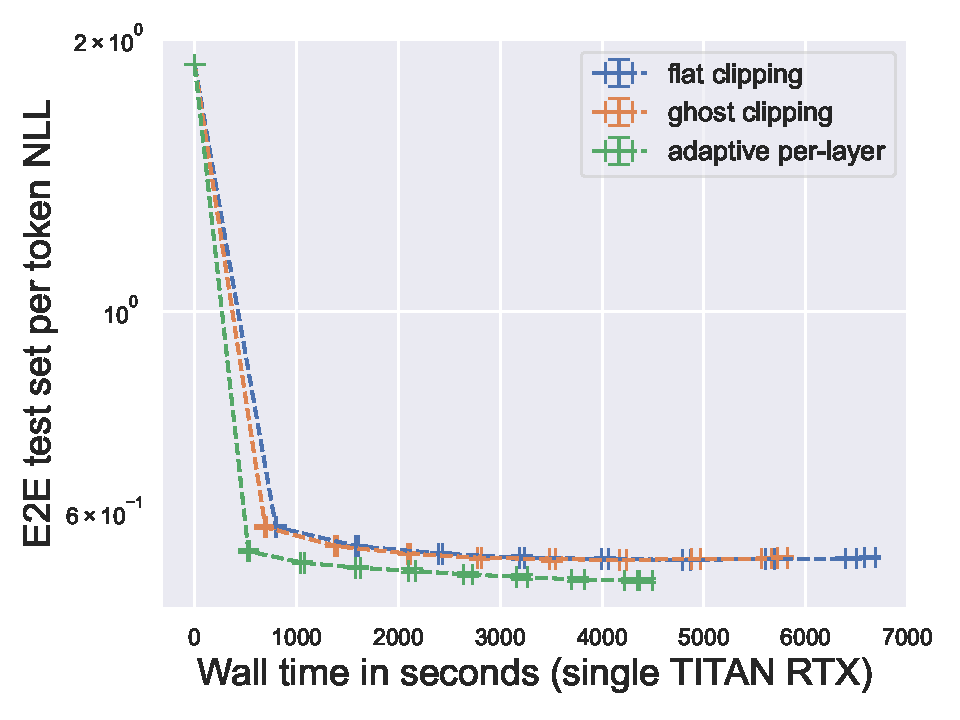
\includegraphics[width=0.95\linewidth]{files/fig/walltime_e2e_test_nll.pdf}} \end{minipage}
\end{center}
\caption{
Adaptive per-layer clipping consistently achieves lower test set negative log-likelihood than flat clipping and ghost clipping under the same wall time.
}
\label{fig:gpt2runtime-overall-nll}
\end{figure}



\begin{figure}[htb]
\begin{center}
\begin{minipage}[t]{0.45\linewidth}
\centering
{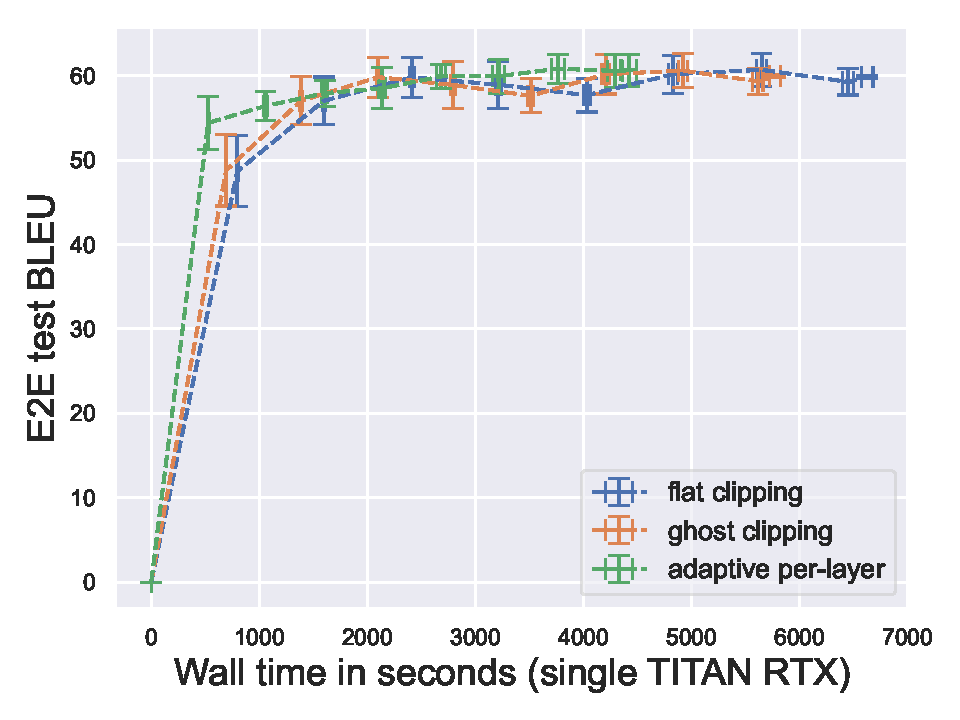
\includegraphics[width=0.95\textwidth]{files/fig/walltime_e2e_test_bleu.pdf}} \\
(a) BLEU
\end{minipage}
\begin{minipage}[t]{0.45\linewidth}
\centering
{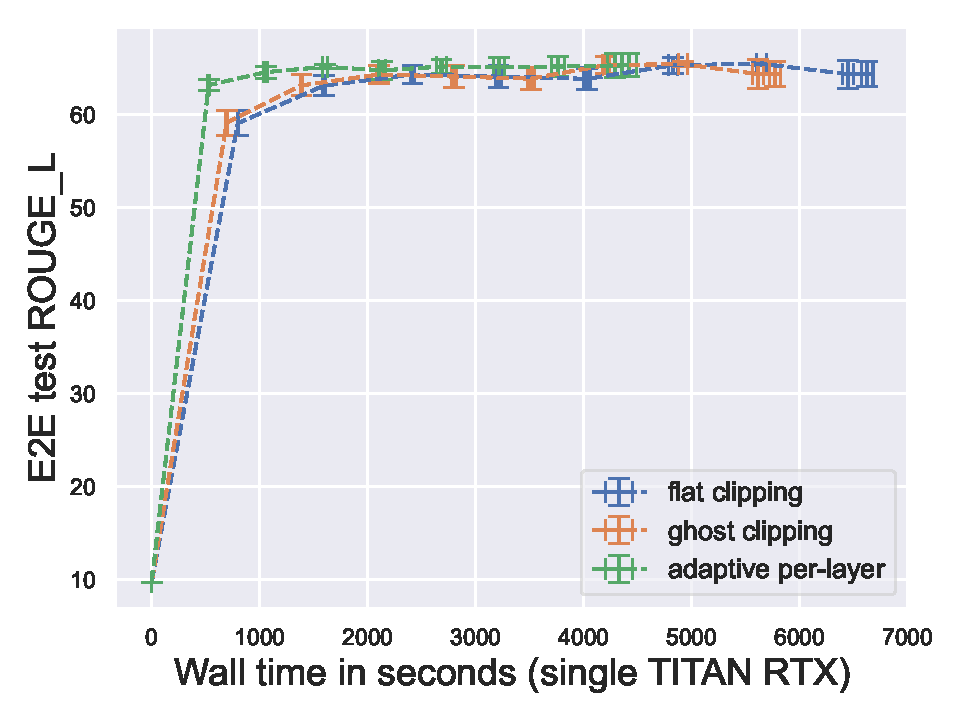
\includegraphics[width=0.95\textwidth]{files/fig/walltime_e2e_test_ROUGE_L.pdf}} \\
(b) ROUGE-L
\end{minipage}
\end{center}
\caption{
Adaptive per-layer clipping generally yields better task metric numbers compared to flat clipping and ghost clipping under the same wall time.
}
\label{fig:gpt2runtime-overall-task-metric}
\end{figure}


\begin{figure}[htb]
\begin{center}
\begin{minipage}[t]{0.45\linewidth}
\centering
{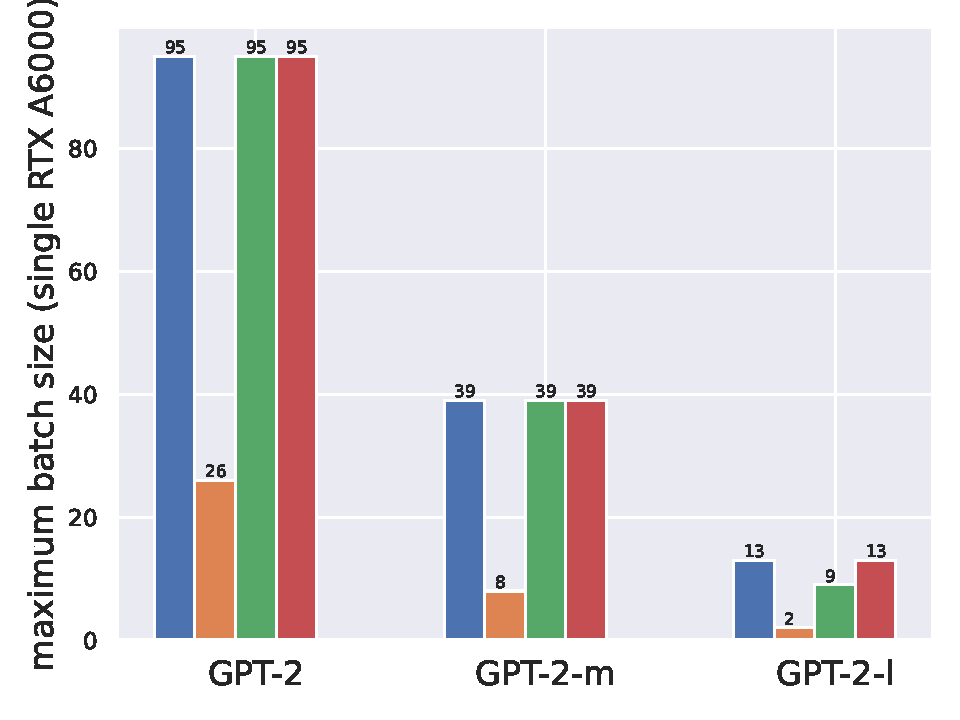
\includegraphics[width=0.95\linewidth]{files/fig/profile_v2/memory_100_default_fast_float.pdf}} \\
(a) Memory
\end{minipage}
\begin{minipage}[t]{0.45\linewidth}
\centering
{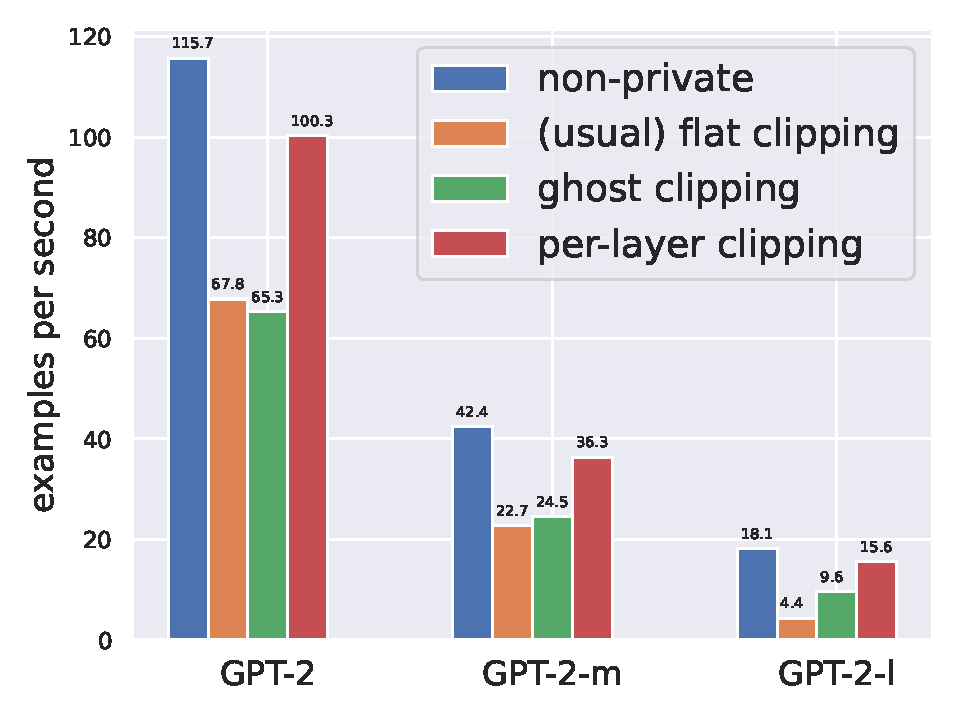
\includegraphics[width=0.95\textwidth]{files/fig/profile_v2/throughput_100_default_fast_float.pdf}} \\
(b) Throughput
\end{minipage}
\end{center}
\caption{
Private learning with (adaptive) per-layer clipping can be almost as efficient as non-private learning (the throughput gap is less than 15\% in this case).
}
\label{fig:gpt2runtime-breakdown}
\end{figure}

